% Intended LaTeX compiler: pdflatex
\documentclass[10pt,a4paper,UTF8]{article}
\usepackage{zclorg}
\author{张朝龙}
\date{}
\title{可逆性与同构}
\hypersetup{
 pdfauthor={张朝龙},
 pdftitle={可逆性与同构},
 pdfkeywords={},
 pdfsubject={},
 pdfcreator={Emacs 25.0.50.1 (Org mode 9.0.5)}, 
 pdflang={English}}
\begin{document}

\maketitle
\tableofcontents
\titlepic{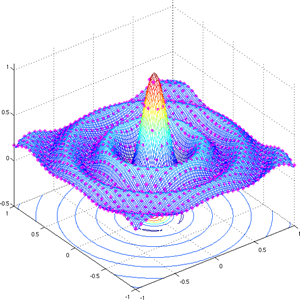
\includegraphics[scale=0.25]{../../img/sinc.PNG}}
在学习 Artin的《抽象代数》过程中,我曾接触过重构的概念。但是我觉得《linear algebra done right》从可逆线性映射到重构的过渡更加的自然,更加适合初学者。
\section{可逆的线性映射}
\label{sec:org81862df}


\begin{definition}
线性映射\(T\in \mathcal{L}(V,W)\)称为可逆的,如果存在线性映射\(S\in \mathcal{L}(W,V)\)使得\(ST\)等于\(V\)上的恒等映射且\(TS\)等于\(W\)上的恒等映射。满足\(ST=I\)和\(TS=I\)的线性映射\(S\in \mathcal{L}(W,V)\)成为\(T\)的逆。
\end{definition}

注意\(ST=I\)的恒等映射是\(W\)上的恒等映射,\(TS=I\)的恒等映射是\(V\)上的恒等映射。
\begin{theorem}
可逆线性映射的逆是唯一的。
\end{theorem}
\begin{proof}
设\(T\in \mathcal{L}(V,W)\)可逆,且\(S_{1}\)和\(S_{2}\)都是\(T\)的逆,则有:
\[S_{1} = S_{1}I = S_{1}(TS_{2}) = (S_{1}T) S_{2} = IS_{2} = S_{2}\]
\end{proof}

由于\(T\)的逆是如此的重要,我们用\(T^{-1}\)来表示\(T\)的逆,即\(TT^{-1} = T^{-1}T = I\)。
\begin{theorem}
一个线性映射是可逆的当且仅当它既是单射又是满射。
\end{theorem}
\begin{proof}
这个命题综合了线性映射,可逆,单射,满射的概念。

首先我们从一个可逆的线性映射推出这个映射既是单射又是满射。假设\(u,v\in V\),且\(Tu=Tv\),则有\(T^{-1}Tu = T^{-1}Tv\)从而有\(u=v\),即\(T\)是单射。假设\(w\in W\),则有\(T(T^{-1}w) = w\),即\(w\in rangeT\),又由于\(w\)的任意性,则有\(rangeT = W\),即\(T\)是满射。

然后,我们从一个线性映射既是单射又是满射推出这个线性映射是可逆的,即对于每个\(w\in W\),定义\(Sw\)是\(V\)中唯一使得\(T(Sw) = w\)的那个元素,显然\(T\circ S\)是\(W\)上的恒等映射。为了证明\(S\circ T\)是\(V\)上的恒等映射,设\(v\in V\),则\[T((S\circ T)v) = (T\circ S)Tv = Tv\]这个等式表明\((S\circ T)v = v\),因此\(S\circ T\)是\(V\)上的恒等映射。

为了完成证明,我们还需要证明\(S\)是线性的。假设\(w_{1},w_{2}\in W\)则有:\[T(Sw_{1} + Sw_{2}) = TSw_{1} + TSw_{2} = w_{1} + w_{2}\]
现在我们知道\(Sw_{1} + Sw_{2}\)是\(V\)中唯一被\(T\)映射成\(w_{1} + w_{2}\)的元素。因为之前我们定义\(Sw\)是\(V\)中唯一使得\(T(Sw) = w\)的那个元素,则有\(S(w_{1} + w_{2}) = w_{1} + w_{2}\)

接下来证明齐次性,如果\(w\in W, \lambda \in \mathbf{F}\),则:\[T(\lambda Sw) = \lambda T(Sw) = \lambda w\]
由于\(T\)是单射所以,\(\lambda Sw\)是唯一被\(T\)映射成\(\lambda w\)的元素。又由于\(S\)的定义\(Sw\)是\(V\)中唯一被\(T\)映射称\(w\)的元素,则有\(S(\lambda w) = \lambda S(w)\)
\end{proof}

\section{向量空间的同构}
\label{sec:org56086f5}


两个向量空间是同构的。意味着,这两个向量空间除了元素名字之外本质上是相同的。这个概念非常重要,因为很多时候我们在一个向量空间中处理问题显得复杂,但是在另外一个空间中则显得简单,所以我们可以在简单的同构空间中先行处理问题,再把处理的结果转换到原空间中。信号处理的时域和频域之间的相互转换就是利用了时域空间和频域空间同构的本质。

\begin{definition}
同构就是可逆的线性映射。若两个向量空间之间存在一个同构,则称这个向量空间是同构的。
\end{definition}

同构\(T:V\rightarrow W\)把\(v\in V\)重新标记为\(Tv\in W\).这个观点解释了为什么两个同构的向量空间具有相同的性质。同构和可逆的线性映射这两个术语的意思相同。同构更强调两个空间本质上的相同。

\begin{theorem}
\(\mathbf{F}\)上两个有限维向量空间同构当且仅当其维数相同。
\end{theorem}
\begin{proof}
设\(V\)和\(W\)是同构的,则存在从\(V\)到\(W\)的同构\(T\)。因为\(T\)是可逆的,所以\(T\)既是单射又是满射,单射意味着\(nullT = \{0\}\),满射意味着\(rangeT = W\),所以\(\dim nullT = 0\), \(\dim range T = \dim W\),根据线性映射基本定理,我们有:\[\dim V = \dim nullT + \dim rangeT = 0 + \dim W\]即,\(\dim V = \dim W\)

接下来,我们证明另一个方向,假定\(V\)和\(W\)是维数相同的向量空间,设\(v_{1},\ldots ,v_{n}\)是\(V\)的基,\(w_{1},\ldots ,w_{n}\)是\(W\)的基。则一定存在线性映射\(T\in \mathcal{L}(V,W)\)定义如下:
\[T(c_{1}v_{1} + \ldots + c_{n}V_{n}) = c_{1}w_{1} + \ldots + c_{n}w_{n}\]
关于这个定义的合理性我们在前面证明过。由于\(w_{1},\ldots ,w_{n}\)张成\(W\),所以\(T\)是满的。又因为\(w_{1},w_{2},\ldots ,w_{n}\)是线性无关的,所以\(nullT = \{0\}\),从而\(T\)是单的。由于\(T\)既是单射又是满射,所以\(T\)是一个同构,因此\(V\)和\(W\)是同构的。
\end{proof}

每个有限维空间都同构与\(\mathbf{F}^{n}\),其中\(n = \dim V\).如果\(v_{1},\ldots ,v_{n}\)是\(V\)的基,\(w_{1},\ldots ,w_{n}\)是\(W\)的基,那么每个\(T\in \mathcal{L}(V,W)\)都有一个矩阵\(\mathcal{M}(T) \in \mathbf{F}^{m,n}\). 也就是说选定了\(V\)和\(W\)的基,那么\(\mathcal{M}\)就是从\(\mathcal{L}(V,W)\)到\(\mathbf{F}^{m,n}\)的函数。

既然每个有限维向量空间都同构于某个\(\mathbf{F}^{n}\),那么为什么不只研究\(\mathbf{F}^{n}\)而还要研究更一般的向量空间呢?我们注意到\(\mathbf{F}^{n}\)的向量空间立刻就会产生不等于\(\mathbf{F}^{n}\)的向量空间。例如我们会遇到线性映射的零空间和值域,尽管这些向量空间都分别同构于某个\(\mathbf{F}^{n}\),但是这样考虑问题会增加不少复杂度。

\begin{theorem}
设\(v_{1},\ldots ,v_{n}\)是\(V\)的基,\(w_{1},\ldots ,w_{m}\)是\(W\)的基,则\(\mathcal{M}\)是\(\mathcal{L}(V,W)\)与\(\mathbf{F}^{m,n}\)之间的一个同构。
\end{theorem}
\begin{proof}
已知\(\mathcal{M}\)是线性的,故只需证明\(\mathcal{M}\)既单又满。先从单性开始,如果\(T\in \mathcal{L}(V,W)\)并且\(\mathcal{M}(T) = 0\),则有\(Tv_{k} = 0,k=1,\ldots ,n\),因为\(v_{1},\ldots ,v_{n}\)是\(V\)的基,所以\(T=0\)。于是\(\mathcal{M}\)是单的(单射的零空间是\(\{0\}\))。

接下来证明\(\mathcal{M}\)是满的,设\(A\in \mathbf{F}^{m,n}\)。设\(T\)是从\(V\)到\(W\)的线性映射使得\[Tv_{k} = \sum_{j=1}^{n}A_{j,k}w_{j}\]其中\(k=1,\ldots ,n\) 显然\(\mathcal{M}(T)\)等于\(A\),所以\(M(T)\)的值域是\(\mathbf{F}^{m,n}\)
\end{proof}

上述定理证明了所有的线性映射都可以映射为\(\mathbf{F}^{m,n}\),所有的\(\mathbf{F}^{m,n}\)都映射为一个线性映射。
\begin{theorem}
\(\dim \mathcal{L}(V,W) = (\dim V)(\dim W)\)
\end{theorem}
\begin{proof}
首先我们知道\(\mathcal{L}(V,W)\)同构于\(\mathbf{F}^{m,n}\),而\(\dim \mathbf{F}^{m,n} = mn\)

然后,\(\dim V = n,\dim W = m\) 

所以结论得证。
\end{proof}

\section{矩阵乘法和线性映射的关系}
\label{sec:orgd56a2a5}


首先,定义向量对应的矩阵:
\begin{definition}
设\(v\in V\),并设\(v_{1},\ldots ,v_{n}\)是\(V\)的基,则规定\(v\)关于这个基的矩阵是\(n\times 1\)矩阵。
\begin{equation}
\label{eq:201703252}
\mathcal{M}(v) = 
\begin{bmatrix}
c_{1} \\ 
\vdots \\
c_{n}
\end{bmatrix}
\end{equation}
这里\(c_{1},\ldots ,c_{n}\)是使得下式成立的标量:
\[v=c_{1}v_{1}+ \ldots + c_{n}v_{n}\] 
\end{definition}

显然,对于\(2-7x+5x^{3}\)关于\(\mathcal{P}_{3}(R)\)的标准基的矩阵为:
\begin{equation}
\label{eq:201703251}
\begin{bmatrix}
2 \\ -7 \\ 0 \\ 5
\end{bmatrix}
\end{equation}

向量\(x\in \mathbf{F}^{n}\)关于标准基的矩阵就是以\(x\)的坐标为元素而得到的\(n\times 1\)矩阵,也即是说,若\(x=(x_{1},\ldots ,x_{n})\in \mathbf{F}^{n}\),则
\begin{equation}
\label{eq:201703253}
\mathcal{M}(x) = 
\begin{bmatrix}
x_{1} \\ \vdots \\ x_{n}
\end{bmatrix}
\end{equation}

以上两个例子都实现了\(V\)到\(\mathbf{F}^{n,1}\)的同构。

\begin{theorem}
设\(T\in \mathcal{L}(V,W)\), \(v_{1},\ldots ,v_{n}\)是\(V\)的基,\(w_{1},\ldots ,w_{m}\)是\(W\)的基。设\(1\leq k \leq n\),则\(\mathcal{M}(T)\)的第\(k\)列(记为\(\mathcal{M}(T)_{\cdot,k}\))等于\(M(Tv_{k})\)
\end{theorem}

\begin{proof}
设\(v=c_{1}v_{1} + \ldots + c_{n}v_{n}\),其中\(c_{1},\ldots ,c_{n}\in \mathbf{F}\),则
\begin{eqnarray}
\label{eq:201703254}
Tv &=& c_{1}Tv_{1} + \ldots + c_{n}Tv_{n} \\
&=& c_{1} \mathcal{M}(T)_{\cdot,1} + \ldots + c_{n} \mathcal{M}(T)_{\cdot,n} \\
&=& \mathcal{M}(T)\mathcal{M}(v)
\end{eqnarray}
\end{proof}
每个\(m\times n\)矩阵\(A\)诱导一个从\(\mathbf{F}^{n,1}\)到\(\mathbf{F}^{m,1}\)的线性映射,即将\(x\in \mathbf{F}^{n,1}\)变为\(Ax\in \mathbf{F}^{m,n}\)的矩阵乘。通过上述命题我们可以知道,利用通过\(\mathcal{M}\),我们可以把线性映射当做矩阵乘映射。具体来说,若\(T\in \mathcal{L}(V,W)\),并将\(v\in V\)等同于\(\mathcal{M}(v)\in \mathbf{F}^{n,1}\),则上述命题说,我们可以将\(Tv\)等同于\(\mathcal{M}(T) \mathcal{M}(v)\).

\section{算子}
\label{sec:org50aa424}


向量空间到其自身的线性映射称为算子。记\(\mathcal{L}(V)\)表示\(V\)上全体算子所组成的集合。即,\(\mathcal{L}(V) = \mathcal{L}(V,V)\) 在线性代数中,最深刻也最重要的内容就是研究算子。

我们知道对于一个线性映射既单又满则可逆,但是对于一个算子是不是也是这样的呢?或者对于一个算子如果仅仅满足单性或者满性是不是也可以推出可逆呢?对于无限维空间我们知道单单一个不能推出可逆性。

\begin{enumerate}
\item \(\mathcal{P}(R)\)上乘以\(x^{2}\)的映射是单的,但不是满的。
\item \(\mathbf{F}^{\infty}\)上向后移位算子是满的,但不是单的。
\end{enumerate}

但是对于有限维向量空间上的算子,单性和满性中的任何一个都可以推出另一个。通常检验有限维向量空间上的算子是单的更容易,而由单性自然可以得到满性。

\begin{theorem}
设\(V\)是有限维的,并设\(T\in \mathcal{L}(V)\),则一下陈述等价:
\begin{enumerate}
\item \(T\)是可逆的;
\item \(T\)是单的;
\item \(T\)是满的;
\end{enumerate}
\end{theorem}

\begin{proof}
显然从 \(T\)是可逆的可以推出\(T\)是单的。

接下来我们假设\(T\)是单的,那么\(nullT = 0\),由线性映射基本定理有:\(rangeT = \dim V - \dim nullT = \dim v\),则有\(\dim V = \dim rangeT\)从而\(T\)是满的。 

最后假设\(T\)是满的,由线性映射基本定理有:\(\dim nullT = \dim V - \dim rangeT = 0\),对出\(T\)是单的,所以\(T\)既单又满是可逆的。
\end{proof}
\end{document}
